% Diese Datei ist Teil des Buchs "Schreibe Dein Programm!"
% Das Buch ist lizensiert unter der Creative-Commons-Lizenz
% "Namensnennung 4.0 International (CC BY 4.0)"
% http://creativecommons.org/licenses/by/4.0/deed.de

\chapter{Programmieren mit Listen}
\label{cha:rek}

Die bisher betrachteten Daten hatten alle immer eine feste Größe~--
die Anzahl der Komponenten zusammengesetzter Daten ist fest, ebenso wie die
Anzahl der Fälle bei Fallunterscheidungen oder gemischten Daten.  Das
reicht nicht für alle Anwendungen: Die Bücher im Regal, die Wagen
eines Zuges, die Fotos im Album sind allesamt in ihrer Anzahl
variabel.  Für die Repräsentation solcher Informationen wird also eine
neue Art der Datendefinition benötigt, welche die schon bekannten
zusammengesetzten und gemischten Daten ergänzt: der
\textit{Selbstbezug}.  Selbstbezüge können benutzt werden, um solche
Daten variabler Größe abzubilden, insbesondere in sogenannten
\textit{Listen}.

\section{Listen repräsentieren}
\label{sec:lists}

\index{Liste}Hier sind einige Listen aus dem täglichen Leben:
%
\begin{center}
  \begin{tabular}{l@{\qquad}l@{\qquad}l@{\qquad}l@{\qquad}l@{\qquad}l}
  Brot & Herbert & 1 & Phidipides & Dauerwelle & Pumps \\
  Butter & Mike & 2 & Diabetes & Dreadlocks \\
  Käse & & 3 & Bursitis & Irokese \\
  & & 4 & Woody & Vokuhila \\
  && 5 & Hepatitis \\
  && 6 & Zeus \\
  &&& Doris\\
  &&& Lorenzo
\end{tabular}
\end{center}
%
Keine dieser Listen ist auf ihre jeweilige Länge festgelegt: Zur Liste
mit "`Brot"' könnten beispielsweise noch "`Gurken"' hinzukommen.  Damit ist es
nicht möglich, diese Listen jeweils durch die bereits bekannten
zusammengesetzten Daten und Records zu repräsentieren, da bei ihnen
die Liste der Komponenten schon in der Datendefinition festgelegt
ist.  Hier kommen Listen im Sinne der Programmierung ins Spiel, die es
erlauben, "`zusammengesetzte Daten variabler Länge"' zu
repräsentieren.  Die einfachste Sorte Liste ist die leere Liste

FIXME
%
\begin{alltt}
(define-record-functions empty-list
  make-empty
  empty?)

(define empty (make-empty))
\end{alltt}
%
Dies ist die \textit{leere Liste}\index{leere
  Liste}\index{Liste!leer}.  Um Listen herzustellen, die nicht leer
sind, dienen \textit{Conse}\index{Cons}, eine besonders allgemein
verwendbare Sorte zusammengesetzter Daten.  Hier sind Daten- und
Record-Definition für Conse:\index{cons@\texttt{cons}}\index{cons@\texttt{cons}}\index{cons?@\texttt{cons?}}\index{first@\texttt{first}}\index{rest@\texttt{rest}}\label{def:cons}
%
\begin{alltt}
; Ein Cons besteht aus:
; - einem beliebigen Element
; - einer Liste
(define-record-functions cons-list
  cons
  cons?
  (first any)
  (rest  a-list))
\end{alltt}
%
Für eine Signatur für den Konstruktor ist es noch zu früh, da es noch
keine Signatur für den Begriff "`Liste"' aus der Datendefinition
gibt.  Diese folgt in wenigen Augenblicken.

Ein Cons kann nun benutzt werden, um die letzte Liste aus der obigen
Tabelle zu repräsentieren.  "`Pumps"' wird als Zeichenkette zum ersten
Element des Cons.  Die \texttt{rest}-Komponente des Cons muß eine
Liste sein~-- dabei ist zu beachten, dass insbesondere die leere Liste
eine Liste ist, dort also verwendet werden kann:
%
\begin{alltt}
(cons "Pumps" empty)
\evalsto{} #<record:cons "Pumps" #<empty-list>>
\end{alltt}
%
Jetzt kommt der entscheidende Punkt: Conse sind \emph{auch} Listen,
Listen sind also gemischte Daten:\index{a-list@\texttt{a-list}}\label{def:a-list}
%
\begin{alltt}
; Eine Liste ist eins der folgenden:
; - die leere Liste
; - ein Cons
(define a-list
  (signature
   (mixed empty-list
          cons-list)))
\end{alltt}
%
Die Signatur \texttt{empty-list} ist bereits eingebaut und paßt auf
die leere Liste \texttt{empty} (und nichts sonst).  (Der Name
\texttt{list} ist in den Lehrsprachen bereits vergeben, darum
heißt die Signatur \texttt{a-list}.)  Jetzt ist es möglich, eine
Signatur für \texttt{cons} sowie die anderen Funktionen der
Record-Definition von \texttt{cons} zu vergeben:
%
\begin{alltt}
(: cons (any a-list -> cons-list))
(: cons? (any -> boolean))
(: first (cons-list -> any))
(: rest (cons-list -> a-list))
\end{alltt}
%
FIXME:

Hinter der Bezeichnung \verb$%a$ verbirgt sich eine 
\emph{Signaturvariable}\index{Signaturvariable}: Sie
steht für eine beliebige Sorte, die aber in den zwei Zeilen, wo sie vorkommt,
die gleiche Sorte darstellen soll.  Damit ist \verb$%a$ etwas anderes als
\texttt{any}, welches erlauben würde, dass die Rückgabesorte von \texttt{first}
verschieden wäre von der Sorte, welche der Konstruktor \texttt{cons} zuvor
verwendet hat.

So weit, so gut: Bisher gab es die leere Liste und eine Liste mit einem
Element.  Wie kommen mehr Elemente in eine Liste?  Indem
\texttt{cons} noch einmal aufgerufen wird:
%
\begin{alltt}
(cons "Mike" (cons "Herbert" empty))
\evalsto{}#<record:cons "Mike" #<record:cons "Herbert" #<empty-list>>>
\end{alltt}
%
Zu einer Liste mit zwei Elementen gehören also zwei Conse.
Entsprechend für drei Elemente:
%
\begin{alltt}
(cons "Brot" (cons "Butter" (cons "Käse" empty)))
\evalsto{}#<record:cons "Brot" #<record:cons "Butter" #<record:cons "Käse" #<empty-list>>>>
\end{alltt}
%
\begin{figure}[tb]
  \centering
  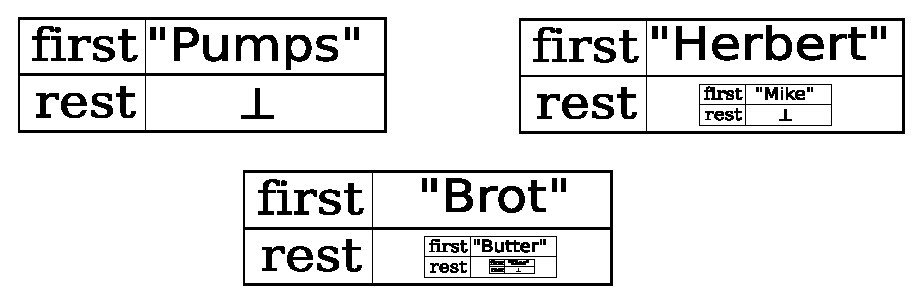
\includegraphics[width=0.8\textwidth]{pair-lists1}
  \caption{Liste mit Consen repräsentiert}
  \label{fig:cons-lists-1}
\end{figure}
Diesmal sind drei Conse im Spiel.  Die Liste wird jeweils
"`terminiert"' durch die leere Liste.  Abbildung~\ref{fig:cons-lists-1}
zeigt, wie die Listen aussehen, wenn sie wie andere zusammengesetzte
Daten als Tabellen dargestellt sind~-- das $\bot$ steht für die leere
Liste. Das sieht aus wie ineinandergeschachtelte russische Puppen und
entspricht damit nicht der gängigen Intuition, wie Listen aufgebaut
sind, aber es funktioniert.  Für viel mehr als drei Elemente
funktioniert die Darstellungsweise allerdings nicht: Darum bevorzugen
wir ab hier sogenannte "`Zeigerdiagramme"', bei denen alle Conse gleich groß
dargestellt sind und ein Pfeil zeigt, dass ein Cons die
\texttt{rest}-Komponente eines anderen Conses bildet.
Abbildung~\ref{fig:cons-lists-2} zeigt das Pfeildiagramm, das
Abbildung~\ref{fig:cons-lists-1} entspricht; es paßt besser zur
gängigen Intuition von Listen.

\begin{figure}[tb]
  \centering
  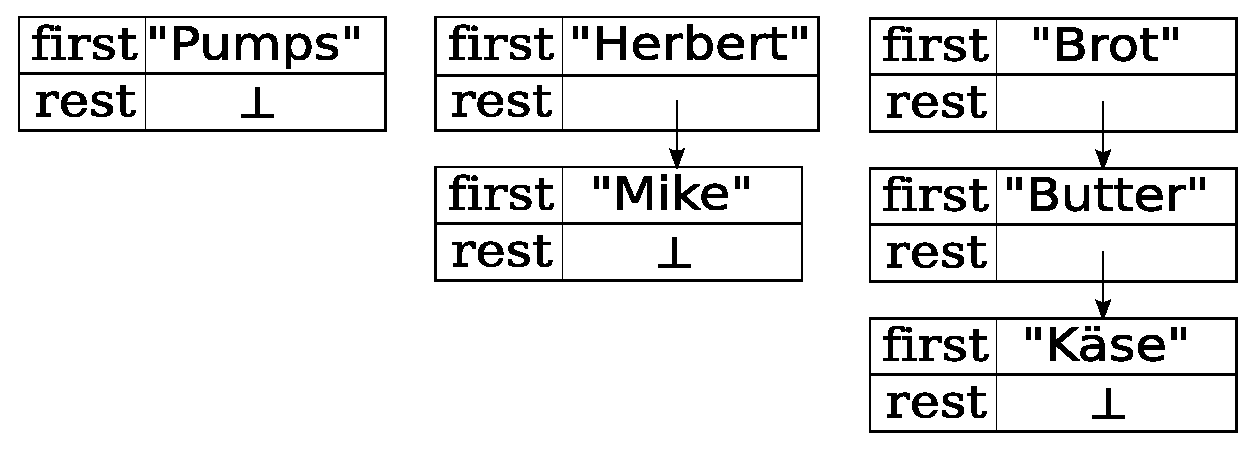
\includegraphics[width=0.8\textwidth]{pair-lists2}
  \caption{Liste mit Consen repräsentiert, als Pfeildiagramm}
  \label{fig:cons-lists-2}
\end{figure}


\section{Mit Listen programmieren}

Als erstes Beispiel für das Programmieren mit Listen schreiben wir
eine Funktion, die eine Liste von Zahlen akzeptiert und deren Summe
liefert.  Dazu werden erst einmal einige Beispiele solcher Listen
benötigt:
%
\begin{verbatim}
; Liste mit den Zahlen 1 2 3
(define n1 (cons 1 (cons 2 (cons 3 empty))))
; Liste mit den Zahlen e und pi
(define n2 (cons 2.7183 (cons 3.14159 empty)))
; Liste mit den Zahlen 2 3 5 7
(define n3 (cons 2 (cons 3 (cons 5 (cons 7 empty)))))
\end{verbatim}

Hier Kurzbeschreibung und Vertrag:\label{sec:list-sum}\index{list-sum@\texttt{list-sum}}
%
\begin{verbatim}
; Summe der Elemente einer Liste von Zahlen berechnen
(: list-sum (a-list -> number))
\end{verbatim}
%
Für die Testfälle halten die Beispiellisten her:
%
\begin{verbatim}
(check-expect (list-sum n1) 6)
(check-within (list-sum n2) 5.85989 0.001)
(check-expect (list-sum n3) 17)
\end{verbatim}
%
Nicht vergessen: In \texttt{n2} sind Zahlen mit Dezimalpunkt.
Deshalb müssen wir \texttt{check-within} verwenden.  Diese Funktion
hat drei Parameter: Die ersten beiden geben ein reales und ein
erwartetes Ergebnis an
und der dritte sagt, um wieviel das reale Ergebnis in der positiven
oder negativen Richtung vom erwarteten Ergebnis abweichen darf. Das Gerüst der
Funktion sieht so aus:
%
\begin{verbatim}
(define list-sum
  (lambda (lis)
    ...))
\end{verbatim}
%
(Es empfiehlt sich, als Bezeichner für Listen nicht einfach nur ein
\texttt{l} zu verwenden, da es in vielen Schriftarten der Ziffer
\texttt{1} ähnlich sieht.)

Zur Erinnerung: Listen sind zunächst gemischte Daten~-- die Definition
von \texttt{a-list} benutzt \texttt{mixed} mit zwei Fällen.  Entsprechend kommt die
Konstruktionsanleitung für gemischte Daten zur Anwendung:
%
\begin{verbatim}
(define list-sum
  (lambda (lis)
    (cond
      (... ...)
      (... ...))))
\end{verbatim}
%
Als nächstes sollten wir die Tests ergänzen, die auf die leere
Liste bzw.\ Conse testen.  Für \texttt{empty} hat dieses Buch Ihnen
den Test bisher vorenthalten: Das eingebaute Prädikat
\texttt{empty?}\index{empty?@\texttt{empty?}} liefert \verb|#t| für
die leere Liste und \verb|#f| für jeden anderen Wert.  Für Conse ist
das Prädikat \texttt{cons?} bereits von der Record-Definition
definiert:
%
\begin{verbatim}
(define list-sum
  (lambda (lis)
    (cond
      ((empty? lis) ...)
      ((cons? lis) ...))))
\end{verbatim}
%
Beim zweiten Zweig des \texttt{cond} handelt es sich um
zusammengesetzte Daten. Ergo ergänzen wir entsprechend der
Konstruktionsanleitung für zusammengesetzte Daten Selektor-Aufrufe in
die Schablone:
%
\begin{verbatim}
(define list-sum
  (lambda (lis)
    (cond
      ((empty? lis) ...)
      ((cons? lis)
       ... (first lis) ... (rest lis) ...))))
\end{verbatim}
%
Jetzt können wir ans Ausfüllen der beiden Zweige gehen: Die erste
Ellipse muß die Frage beantworten, was die Summe der leeren Liste sein
soll.  Diese Frage ist bei nahezu \emph{allen} Funktionen relevant,
die Listen akzeptieren, es empfiehlt sich darum grundsätzlich, einen
Testfall für die leere Liste zu formulieren:
%
\begin{alltt}
(check-expect (list-sum empty) \textrm{?})
\end{alltt}
%
Die Antwort ist nicht ganz offensichtlich, wir können 
sie aber durch folgende Überlegung gewinnen: Betrachten wir Listen aus
Einsen, dann entspricht deren Summe immer der Länge der Liste.  Wenn
die Liste leer ist hat sie die Länge $0$, entsprechend ist also auch
ihre Summe $0$:
%
\begin{alltt}
(check-expect (list-sum empty) 0)
\ldots
(define list-sum
  (lambda (lis)
    (cond
      ((empty? lis) 0)
      ((cons? lis)
       ... (first lis) ... (rest lis) ...))))
\end{alltt}
%
Bleibt der zweite Zweig mit den Consen.  Hier hilft es, die beiden
Selektor-Aufrufe \texttt{(first lis)} und \texttt{(rest lis)} auf die
Daten zurückzubeziehen.  \texttt{(first lis)} liefert für die drei
Beispiellisten folgende Werte:
%
\begin{alltt}
(first n1)
\evalsto{} 1
(first n2)
\evalsto{} 2.7183
(first n3)
\evalsto{} 2
\end{alltt}
%
Das ist jeweils das \emph{erste Element}~-- kein Wunder, dass der
Selektor \texttt{first}\index{first@\texttt{first}} heißt.  Nun für \texttt{rest}\index{rest@\texttt{rest}}:
%
\begin{alltt}
(rest n1)
\evalsto{} #<record:cons 2 #<record:cons 3 #<empty-list>>>
(rest n2)
\evalsto{}  #<record:cons 3.14159 #<empty-list>>
(rest n3)
\evalsto{} #<record:cons 3 #<record:cons 5 #<record:cons 7 #<empty-list>>>>
\end{alltt}
%
Dies sind jeweils Listen mit allen Elementen \emph{außer dem
  ersten}, also quasi den \emph{Rest}~-- daher der Name \texttt{rest}
für den Selektor.

Zurück zur Schablone: Was können wir mit dem ersten Element der Liste
und dem Rest der Liste anfangen?  Hier kommt ein besonderer Trick zum
Zug~-- da der Rest der Liste wieder eine Liste ist, können
wir von der Summe des Rests sprechen.  Wenn diese Summe bekannt
ist~-- also \emph{die Summe aller Elemente außer des ersten}, dann
könnten wir (und das Programm auch) die Gesamtsumme ermitteln, indem wir
auf diese Summe das noch fehlende erste Element addieren.  "`Die Summe
aller Elemente außer des ersten"' können wir so aufschreiben:
%
\begin{alltt}
(list-sum (rest lis))
\end{alltt}
%
Entsprechend die Summe des ersten Elements und der Summe des Rests:
%
\begin{alltt}
(+ (first lis) (list-sum (rest lis)))
\end{alltt}
%
Das können wir in die Schablone von oben einsetzen:
%
\begin{verbatim}
(define list-sum
  (lambda (lis)
    (cond
      ((empty? lis) 0)
      ((cons? lis)
       (+ (first lis) (list-sum (rest lis)))))))
\end{verbatim}
%
Dieses Programm ist nicht nur vollständig, es funktioniert auch
tatsächlich: Alles was wir gemacht haben war, die Kurzbeschreibung
von \texttt{list-sum} ernst zu nehmen, die behauptet, dass die Funktion
die Summe einer beliebigen Liste berechnet: \texttt{(rest lis)} ist
eine Liste, also kann \texttt{list-sum} auch deren Summe berechnen.

Um den "`Selbstaufruf"' von \texttt{list-sum} noch besser zu
verstehen, betrachten wir noch einmal die Datendefinition für
Listen zusammen mit der Datendefinition für Conse:

\begin{pspdf}
\begin{ttfamily}\obeylines
; Eine \rnode[r]{ListeDef}{\textbf{Liste}} ist eins der folgenden:
; - die leere Liste
; - ein Cons
; Ein Cons besteht aus:
; - einem beliebigen Element
; - einer \rnode[r]{ListeRef}{\textbf{Liste}}\nccurve[nodesep=3pt]{->}{ListeRef}{ListeDef}
\end{ttfamily}
\end{pspdf}

Die Datendefinition enthält einen Verweis auf \emph{sich selbst},
genannt \emph{Selbstbezug}\index{Selbstbezug}.  Dieser Selbstbezug ist
beim Rest~-- der Selbstaufruf, der in \texttt{list-sum} auf den Rest
erfolgt, folgt also der Datendefinition.  Ein Selbstaufruf
heißt auch \textit{rekursiver Aufruf}\index{rekursiver Aufruf} und ist
damit fester Bestandteil der Schablone für Funktionen, die Listen
akzeptieren:
%
\begin{alltt}
(: \textit{proc} (a-list -> ...))

(define \textit{proc}
  (lambda (lis)
    (cond
      ((empty? lis) ...)
      ((cons? lis)
       ... (first lis)
       ... (\textit{proc} (rest lis)) ...))))
\end{alltt}
%
Jetzt wo wir die Schablone haben, gehen wir noch ein weiteres Beispiel
durch, bei dem wir sie von vornherein anwenden:  Gefragt ist eine
Funktion, die eine Liste von Zahlen akzeptiert und feststellt, ob alle
Listenelemente  positiv sind.  Die Funktion beantwortet eine
Ja/Nein-Frage, die damit auch die Kurzbeschreibung bildet:
%
\begin{alltt}
; sind alle Zahlen aus einer Liste positiv?
\end{alltt}
%
Hier ist der dazu passende Vertrag:\index{all-positive?@\texttt{all-positive?}}
%
\begin{verbatim}
(: all-positive? (a-list -> boolean))
\end{verbatim}
%
Für Testfälle stehen die leere Liste sowie die drei Beispiellisten
\texttt{n1}, \texttt{n2} und \texttt{n3} aus dem vorherigen Beispiel
zur Verfügung:
%
\begin{verbatim}
(check-expect (all-positive? empty) #t)
(check-expect (all-positive? n1) #t)
(check-expect (all-positive? n2) #t)
(check-expect (all-positive? n3) #t)
\end{verbatim}
%
Der \texttt{empty}-Testfall ist vielleicht etwas verwirrend: In der
Tat sind alle Elemente der leeren Liste positiv.  Eine andere Art dies
zu sagen wäre, dass kein Element der leeren Liste nicht positiv ist.

Diese Testfälle reichen sichtlich nicht aus, da alle \verb|#t| ergeben
sollen: Diese würden auch von folgender Funktion erfüllt:
%
\begin{verbatim}
(define all-positive?
  (lambda (lis)
    #t))
\end{verbatim}
%
Also werden noch Beispiele mit nicht-positiven Elementen benötigt~--
insbesondere eins mit dem Grenzfall $0$:
\begin{verbatim}
(check-expect (all-positive? (cons -5 empty)) #f)
(check-expect (all-positive? (cons 0 empty)) #f)
(check-expect (all-positive? (cons 1 (cons -2 empty))) #f)
\end{verbatim}
%
Das Gerüst ist wie folgt:
%
\begin{verbatim}
(define all-positive?
  (lambda (lis)
    ...))
\end{verbatim}
%
Wir können nun die Schablone für Listen direkt benutzen:
%
\begin{verbatim}
(define all-positive?
  (lambda (lis)
    (cond
      ((empty? lis) ...)
      ((cons? lis)
       ... (first lis)
       ... (all-positive? (rest lis)) ...))))
\end{verbatim}
%
Das Ergebnis im ersten Zweig wird durch den ersten Testfall diktiert:
\verb|#t|.  Wie schon zuvor machen wir uns die Bedeutung der
Ausdrücke im \texttt{cons}-Zweig klar:
\texttt{(first lis)} ist das erste Element der Liste.
\texttt{(all-positive? (rest lis))} besagt, ob alle Elemente
des Rests von \texttt{lis} positiv sind.  Es sind nur dann alle
Elemente von \texttt{lis} positiv, wenn \texttt{(first lis)}
positiv ist \emph{und} \texttt{(all-positive? (rest lis))} als Ergebnis
\verb|#t| liefert.  Damit ist klar, wie die beiden Ausdrücke
kombiniert werden müssen:
%
\begin{verbatim}
(define all-positive?
  (lambda (lis)
    (cond
      ((empty? lis) #t)
      ((cons? lis)
       (and (> (first lis) 0)
            (all-positive? (rest lis)))))))
\end{verbatim}
%
Konstruktionsanleitung~\ref{ka:listen} auf Seite~\pageref{ka:listen}
faßt die Schablone für Funktionen, die Listen akzeptieren, noch einmal
zusammen.

\section{Signaturkonstruktoren}

Die Beispiellisten vom Anfang dieses Kapitels sind allesamt
\textit{homogen}\index{homogen}: Alle Elemente der Liste sind jeweils
von derselben Sorte.  Es gibt eine Liste von Essenszutaten, eine von
Eigennamen, eine von Zahlen, eine von dramatischen Figuren, eine von
Frisuren und eine von Schuhen.  Die Datendefinition für
\texttt{a-list} von Seite~\ref{def:a-list} ist da allerdings nicht
festgelegt: es heißt ausdrücklich, dass jedes Cons ein
\emph{beliebiges} Element enthält.  So ist beispielsweise auch
folgende Liste zulässig:
%
\begin{verbatim}
(: ml1 a-list)
(define ml1 (cons 5 (cons "Herbert" empty)))
\end{verbatim}
%
In den meisten Fällen gehören jedoch alle Elemente einer Liste zu
derselben Sorte beziehungsweise haben dieselbe Signatur: Schön wäre
es, wenn die Signatur für die Liste dokumentieren könnte, welche
Signatur die Elemente haben.  Wir könnten bei
der Definition von \texttt{cons} die Signatur der Elemente angeben,
also \texttt{cons} zum Beispiel auf Elemente der Signatur
\texttt{number} fest abonnieren: 
%
\begin{alltt}
(define-record-functions cons-list
  cons
  cons?
  (first number)
  (rest  list-of-numbers))
(: cons (number list-of-\textbf{numbers} -> cons))
(: cons? (any -> boolean))
(: first (cons -> \textbf{number}))
(: rest (cons -> list-of-\textbf{numbers}))
\end{alltt}
%
Entsprechend würden wir die daraus resultierende Signatur für Listen
nicht mehr \texttt{a-list} sondern \texttt{list-of-numbers} nennen:\index{list-of-numbers@\texttt{list-of-numbers}}
%
\begin{verbatim}
(define list-of-numbers
  (signature
   (mixed empty-list
          cons-list)))
\end{verbatim}
%

FIXME

Mit
\texttt{define-record-functions} können wir die
Record-Definition von \texttt{cons} erweitern:
%
\begin{verbatim}
(define-record-functions (cons-of a)
  cons cons?
  (first a)
  (rest (list-of a)))
\end{verbatim}
%
\texttt{Cons-of} ist der Signaturkonstruktor.  (Das angehängte
\texttt{-of} ist, ähnlich wie das \texttt{make-} bei den
Konstruktoren, das \texttt{?} beim Prädikat und den Feld-Namen bei den
Selektoren reine Konvention.)

Konstruktor, Prädikat
und Selektoren für das neue \texttt{cons} haben die folgenden
Signaturen:
%
\begin{verbatim}
(: cons (%a (list-of %a) -> (cons-of %a)))
(: cons? (any -> boolean))
(: first ((cons-of %a) -> %a))
(: rest ((cons-of %a) -> (list-of %a)))
\end{verbatim}
%
Hier ist  \verb|%a| eine
\textit{Signaturvariable}, die für eine beliebige
Signatur steht, die erst beim Aufruf von \texttt{cons} beziehungsweise
\texttt{first} oder \texttt{rest} festgelegt wird.
Die Tatsache, dass hier zwei verschiedene Signaturvariablen
verwendet wurden bringt die zusätzliche Information für den
menschlichen Leser zum Ausdruck, dass die
Argumente von \texttt{cons-of} zu potentiell
unterschiedlichen Signaturen gehören.

Zu lesen sind die obigen Signaturdeklarationen so:
%
\begin{itemize}
\item \texttt{cons} akzeptiert zwei Argumente beliebiger Signaturen
  \verb|%a| und \verb|%b| und
  liefert als Resultat einen Record, dessen erstes Feld von der Signatur
  \verb|%a| und dessen zweites Feld von der Signatur \verb|%b| ist.
\item Das Resultat von \texttt{first} hat die
  Signatur des ersten Feldes seines Arguments.
\item Das Resultat von \texttt{rest} hat die
  Signatur des zweiten Feldes seines Arguments.
\end{itemize}
%

Diese Signaturen sind allerdings noch unbefriedigend, da sie nicht zum
Ausdruck bringen, dass das zweite Argument von \texttt{cons} immer
eine \emph{Liste} sein muß beziehungsweise daß \texttt{rest} immer
eine Liste liefert.  Diese Problematik stellen wir noch einen Moment
hintenan, werden aber später zu ihr zurückkehren~-- zunächst einmal zu
den Signaturen für Listen.

FIXME

Mit Hilfe von \texttt{cons-of} können wir versuchen, einen Ersatz für
\texttt{a-list} zu definieren, der spezifiziert, auf welche Signatur
die Elemente der Liste passen.  Das könnte so aussehen:
%
\begin{alltt}
(define list-of-numbers
  (signature
    (mixed empty-list
           (cons-of \textbf{number} list-of-numbers))))
\end{alltt}
%
Entsprechend für Zeichenketten:
%
\begin{alltt}
(define list-of-strings
  (signature
    (mixed empty-list
           (cons-of \textbf{string} list-of-strings))))
\end{alltt}
%
Wie schon oben angemerkt, wäre es unbefriedigend, für jede Elementsignatur eine
eigene Listensignatur definieren zu müssen, immer auf die gleiche
Weise.  Aber glücklicherweise unterscheiden sich
\texttt{list-of-numbers} und \texttt{list-of-strings} nur an einer
einzigen Stelle, und über die können wir abstrahieren:
%
\begin{verbatim}
(define list-of
  (lambda (x)
    (signature
      (mixed empty-list
             (cons-of x)))))
\end{verbatim}
%
Fertig!  Nun können wir Signaturen für Listen von Zahlen als
\texttt{(list-of number)}, Listen von Zeichenketten als
\texttt{(list-of string)} und Listen von beliebigen Werten als
\texttt{(list-of any)} schreiben.  Außerdem können wir diese
Definition jetzt verwenden, um bessere Signaturen für
\texttt{cons}, \texttt{first} und \texttt{rest} anzugeben:
%
\begin{verbatim}
(: cons (%a (list-of %a) -> (cons-of %a)))
(: cons? (any -> boolean))
(: first ((cons-of %a) -> %a))
(: rest ((cons-of %a) -> (list-of %a)))
\end{verbatim}
%

\section{Eingebaute Listen}

Da Listen in diesem Buch noch oft vorkommen und es umständlich
ist, jedesmal die Definitionen für \texttt{cons} und \texttt{list-of} an den Anfang
von Programmen zu setzen, ist es an dieser Stelle Zeit, eine neue
Sprachebene in \drscheme{} auszuwählen, nämlich \texttt{Schreibe Dein Programm!}
(ohne \texttt{Anfänger}).\index{Sprachebene}  Diese enthält \texttt{cons},
\texttt{cons?}, \texttt{first} und \texttt{rest} als eingebaute
Funktionen sowie den Signaturkonstruktor \texttt{list-of}\footnote{In Standard-Scheme heißt der Konstruktor für
  die eingebauten Conse \texttt{cons\index{cons@\texttt{cons}}}, die
  Selektoren \texttt{car\index{car@\texttt{car}}} und \texttt{cdr\index{cdr@\texttt{cdr}}}
  (gesprochen "`kar"' und "`kudder"'; dies waren die Namen von Anweisungen auf einer
  Maschine, auf der ein Vorläufer von Scheme lief) und das Prädikat
  für die leere Liste \texttt{null?\index{null?@\texttt{null?}}}.} und eine
eingebaute Funktion \texttt{list} zur Erzeugung beliebiger Listen.

Außerdem werden nichtleere Listen ab dieser Sprachebene in der REPL
anders ausgedruckt, nämlich, der besseren Übersicht halber, als
\verb|#<list ...>|,
wobei die Listenelemente zwischen den spitzen Klammern aufgereiht sind.
Beispiele:

\begin{alltt}
(list 1)
\evalsto{} #<list 1>
(list 1 2)
\evalsto{} #<list 1 2>
(list 1 2 3)
\evalsto{} #<list 1 2 3>
\end{alltt}
%
\begin{feature}{\texttt{list}}{scheme:list}
  Die eingebaute Funktion \texttt{list}\index{list@\texttt{list}} erlaubt es, Listen aus ihren Elementen
  ohne Verwendung von \texttt{cons} zu erzeugen.  Sie
  akzeptiert eine beliebige Anzahl von Argumenten, macht daraus eine
  Liste und gibt diese zurück:
%
\begin{alltt}
(list 1 2 3)
\evalsto{} #<list 1 2 3>
(list "Axl" "Slash" "Izzy")
\evalsto{} #<list "Axl" "Slash" "Izzy">
\end{alltt}
\end{feature}


\section{Parametrische Polymorphie}
\label{sec:parametric-polymorphism}
\label{sec:more-lists}

In diesem Abschnitt programmieren wir eine Funktion, welche die Länge
einer Liste ermittelt.\index{list-length@\texttt{list-length}} Das ist
eine einfache Fingerübung mit einer interessanten Eigenschaft.  Hier
sind Kurzbeschreibung und Signatur:
%
\begin{alltt}
; Länge einer Liste berechnen
(: list-length ((list-of %a) -> natural))
\end{alltt}
%
FIXME:

Dieser Funktion ist egal, welche Signatur
die Elemente der Liste erfüllen, weil das Konzept der Länge einer
Liste unabhängig davon ist, was die Elemente sind.
Dementsprechend steht dort nur die Signaturvariable \verb|%a|.
Solche Funktionen, die Argumente akzeptieren, deren Signaturen
Signaturvariablen enthalten, heißen \textit{polymorph} oder auch
\textit{parametrisch polymorph} (weil die Signaturvariable eine Art
Parameter abgibt), und das dazugehörige Konzept heißt
\textit{parametrische
  Polymorphie}\index{Polymorphie}\index{parametrische Polymorphie}:
ein großes Wort, das hier für eine kleine Sache steht.  Interessantere
Beispiele für parametrische Polymorphie wird es in
Kapitel~\ref{cha:higher-order} geben.

Weiter mit \texttt{list-length}~-- hier ist das Gerüst:
%
\begin{alltt}
(define list-length
  (lambda (lis)
    ...))
\end{alltt}
%
Die Schablone ist wie gehabt:
%
\begin{alltt}
(define list-length
  (lambda (lis)
    (cond
      ((empty? lis) ...)
      ((cons? lis) 
       ... (first lis) ...
       ... (list-length (rest lis)) ...))))
\end{alltt}
%
Es ist \texttt{list-length} egal, was der Wert von \texttt{(first
  lis)} ist.  Die Länge der Liste ist unabhängig davon, was für Werte
sich darin befinden: entscheidend ist nur, wieviele es sind.  (Dieser
Umstand ist gerade verantwortlich für die parametrische Polymorphie.)
Damit können wir \texttt{(first lis)} aus der Schablone streichen und
diese dann zum vollständigen Rumpf ergänzen:
%
\begin{alltt}
(define list-length
  (lambda (lis)
    (cond
      ((empty? lis) 0)
      ((cons? lis) 
       (+ 1 
          (list-length (rest lis)))))))
\end{alltt}
%

\section{Funktionen, die Listen produzieren}

In den vorherigen Abschnitten haben wir ausschließlich Funktionen
programmiert, die Listen \emph{akzeptieren}.  In diesem Abschnitt
schreiben wir Funktionen, die Listen \emph{produzieren}.  Das geht mit
Techniken, die wir bereits vorgestellt haben.  Wir machen die Sache
interessanter, indem wir in einem ersten Beispiel Listen von
zusammengesetzten Daten betrachten und in einem zweiten Beispiel zwei
Listen verarbeiten.

\subsection{Gürteltiere überfahren}

Auf Seite~\pageref{page:run-over-dillo} haben wir die Funktion
\texttt{run-over-dillo} geschrieben, die für das Überfahren von
Gürteltieren zuständig ist.  In diesem Abschnitt schreiben wir die
Funktion, die das gleich massenweise erledigt, beispielsweise für alle
Gürteltiere auf einem Highway.  Dazu übernehmen wir Daten- und
Record-Definition von Gürteltieren aus
Abschnitt~\ref{page:run-over-dillo} sowie die Funktiondefinition von
\texttt{run-over-dillo}.  Gürteltiere können wir in Listen stecken,
ebenso wie Zahlen, Zeichenketten oder boolesche Werte.  Hier ist ein
Beispiel:
%
\begin{verbatim}
; Gürteltiere auf Highway 75
(define dl75 (list d1 d2 d3 d4))
\end{verbatim}
(\texttt{D1}, \texttt{d2}, \texttt{d3} und \texttt{d4} sind die
Beispielgürteltiere aus Abschnitt~\ref{page:run-over-dillo}.)

Diese Liste hat die Signatur \texttt{(list-of dillo)}.  Wenn wir eine
Funktion schreiben wollen, die alle Gürteltiere aus einer Liste
überfährt, müßte diese also folgende Kurzbeschreibung und Signatur
haben:
%
\begin{verbatim}
; Gürteltiere überfahren
(: run-over-dillos ((list-of dillo) -> (list-of dillo)))
\end{verbatim}
%
Als Testfall kann obige Beispielliste herhalten:
%
\begin{verbatim}
(check-expect (run-over-dillos dl75)
              (list (make-dillo 55000 #f)
                    d2
                    (make-dillo 60000 #f)
                    d4))
\end{verbatim}
%
Zur Erinnerung: \texttt{d2} und \texttt{d4} sind bereits tot,
dementsprechend sind sie überfahren wie zuvor.

Hier ist das Gerüst:
%
\begin{verbatim}
(define run-over-dillos
  (lambda (dls)
    ...))
\end{verbatim}
%
Die Funktion akzeptiert eine Liste als Eingabe, wir können also, wie
schon so oft, die entsprechende Schablone zum Einsatz bringen:
%
\begin{verbatim}
(define run-over-dillos
  (lambda (dls)
    (cond
     ((empty? dls) ...)
     ((cons? dls)
      ... (first dls) ...
      ... (run-over-dillos (rest dls)) ...))))
\end{verbatim}
%
Im ersten Zweig ist die Sache klar: Geht eine leere Liste rein, kommt
auch eine leere Liste raus.  Im zweiten Zweig können wir uns erst
einmal um das erste Gürteltier kümmern.  Wir haben ja bereits eine
Funktion, die ein einzelnes Gürteltier überfährt; diese können wir auf
das erste Element der Liste anwenden:
%
\begin{verbatim}
(define run-over-dillos
  (lambda (dls)
    (cond
     ((empty? dls) empty)
     ((cons? dls)
      ... (run-over-dillo (first dls)) ...
      ... (run-over-dillos (rest dls)) ...))))
\end{verbatim}
%
Lesen wir noch einmal die beiden Ausdrücke, die im zweiten Zweig
stehen:
%
\begin{itemize}
\item \texttt{(run-over-dillo (first dls))} ist das erste Gürteltier
  der Liste, überfahren.
\item \texttt{(run-over-dillos (rest dls))} ist eine Liste der
  restlichen Gürteltiere, überfahren.
\end{itemize}
%
Gefragt ist eine Liste \emph{aller} Gürteltiere, überfahren:
Wir müssen also nur die Resultate der beiden Ausdrucke mit
\texttt{cons} kombinieren:
%
\begin{verbatim}
(define run-over-dillos
  (lambda (dls)
    (cond
     ((empty? dls) empty)
     ((cons? dls)
      (cons (run-over-dillo (first dls))
                 (run-over-dillos (rest dls)))))))
\end{verbatim}
%
Fertig!

Dieses Beispiel zeigt, dass wir für Funktionen, die Listen produzieren,
keine neue Technik brauchen: Wenn eine Funktion eine leere Liste
produzieren soll, benutzen wir an der entsprechenden Stelle
\texttt{empty}, und bei nichtleeren Listen benutzen wir
\texttt{cons}, bringen also die Schablone für Funktionen zum
Einsatz, die zusammengesetzte Daten produzieren.

\subsection{Zwei Listen aneinanderhängen}
In unserem nächsten Beispiel ist eine Funktion
\texttt{concatenate}\index{concatenate@\texttt{concatenate}} gefragt, die zwei
Listen aneinanderhängt:\label{sec:concatenate}
% 
\begin{alltt}
(concatenate (list 1 2 3) (list 4 5 6))
\evalsto{} #<list 1 2 3 4 5 6>
\end{alltt}
%
Kurzbeschreibung, Signatur und Gerüst sehen folgendermaßen aus:\index{concatenate@\texttt{concatenate}}
%
\begin{alltt}
; zwei Listen aneinanderhängen
(: concatenate ((list-of %a) (list-of %a) -> (list-of %a)))
(define concatenate
  (lambda (lis-1 lis-2)
    ...))
\end{alltt}
%
Die Konstruktionsanleitung aus Abschnitt~\ref{sec:lists} ist
eigentlich nur für Funktionen gedacht, die eine einzelne Liste
akzeptieren.  Welche von beiden ist das $l$ aus der Anleitung?  Im
Zweifelsfall können wir beide Alternativen ausprobieren.  Wir
fangen, um die Sache spannender zu machen, mit \texttt{lis-2} an:
%
\begin{alltt}
(define concatenate
  (lambda (lis-1 lis-2)
    (cond
      ((empty? lis-2) ...)
      ((cons? lis-2) 
       ... (first lis-2)
       ... (concatenate lis-1 (rest lis-2)) ...))))
\end{alltt}
%
Der erste Zweig des \texttt{cond} ist noch einfach: Wenn
\texttt{lis-2} leer ist, muß \texttt{lis-1} herauskommen.  Jedoch wäre für
das obige Beispiel der Wert von \texttt{(concatenate lis-1 (rest lis-2))} die
folgende Liste:
%
\begin{alltt}
#<list 1 2 3 5 6>
\end{alltt}
%
Bei dieser Liste fehlt das
Element 4 in der Mitte, und es ist nicht ersichtlich, wie unsere Funktion
sie passend ergänzen könnte.  Diese
Möglichkeit führt also in eine Sackgasse. Wir versuchen deshalb, die Schablone  auf
\texttt{lis-1} 
 statt auf \texttt{lis-2} anzuwenden:
%
\begin{alltt}
(define concatenate
  (lambda (lis-1 lis-2)
    (cond
      ((empty? lis-1) ...)
      ((cons? lis-1) 
       ... (first lis-1)
       ... (concatenate (rest lis-1) lis-2) ...))))
\end{alltt}
%
Die erste Ellipse ist einfach zu ersetzen:  Ist die erste Liste
leer, ist das Ergebnis die zweite Liste \texttt{lis-2}.  Für den
zweiten Fall sollten wir uns noch einmal ins Gedächtnis rufen,
was für einen Wert \texttt{(concatenate (rest lis-1) lis-2)} liefert: das Ergebnis
dieses Aufrufs ist eine
Liste, die aus \texttt{(rest lis-1)} und \texttt{lis-2} zusammengesetzt
wurde.  Auf das obige Beispiel übertragen, mit \texttt{lis-1} $=$
\verb|#<list 1 2 3>| und \texttt{lis-2} $=$
\verb|#<list 4 5 6>|, ist \texttt{(rest lis-1)} $=$ \verb|#<list 2 3>|.
Der Wert von \texttt{(concatenate (rest lis-1) lis-2)} wäre
also:
%
\begin{alltt}
#<list 2 3 4 5 6>
\end{alltt}
%
Es fehlt das erste Element von \texttt{lis-1}, \texttt{(first
  lis-1)}, das vorn an das Ergebnis angehängt werden muß.  Das geht
mit \texttt{cons}:
%
\begin{alltt}
(define concatenate
  (lambda (lis-1 lis-2)
    (cond
      ((empty? lis-1) lis-2)
      ((cons? lis-1) 
       (cons (first lis-1)
                  (concatenate (rest lis-1) lis-2))))))
\end{alltt}
%
Dieses Beispiel zeigt ein weiteres Schablonenelement, das noch öfter
vorkommen wird:  Wie bei anderen zusammengesetzten Daten müssen Funktionen, die
Listen konstruieren sollen, irgendwo ein \texttt{cons} enthalten.

\texttt{List-length} und \texttt{concatenate} sind gute
Programmierübungen.  Da viele Programme diese Operationen benötigen,
sind sie in den Lehrsprachen  bereits unter den Namen
\texttt{length}\index{length@\texttt{length}} und
\texttt{append}\index{append@\texttt{append}} eingebaut.


\section*{Anmerkungen}

Listen sind, was Datenstrukturen betrifft, eine Art Alleskleber:
Sie taugen auch für die Repräsentation von Tabellen,
Mengen und vielen anderen zusammengesetzten Daten.  Für Listen gibt es
eine riesige Anzahl praktischer Funktionen, von denen die Funktionen in
diesem Kapitel nur die Spitze des Eisberges sind.  Da 
ab hier Listen in den Lehrsprachen fest eingebaut sind, können sie als universelles
Kommunikationsmittel zwischen Programmen dienen, weil sich Funktionen
auf Listen aus einem Programm auch in einem anderen verwenden lassen.
Dies unterscheidet funktionale Sprachen von vielen anderen Programmiersprachen, in
denen Listen vom Programmierer selbst definiert werden müssen oder nur
eine untergeordnete Rolle spielen.

Viele andere Programmiersprachen bauen auf \textit{Felder\index{Feld}} oder
\textit{Arrays\index{Array}} als fundamentale Datenstrukturen für die
Repräsentation von Folgen.  Diese gibt es in
Scheme auch (unter dem Namen \textit{Vektor\index{Vektor}}), finden jedoch
nur selten Verwendung: Oft läßt sich eine
bessere Lösung mit Listen oder anderen Repräsentationen finden.

\section*{Aufgaben}

\begin{aufgabe}
  Schreiben Sie Ausdrücke für Listen, welche die Beispiellisten vom
  Anfang von Abschnitt~\ref{sec:lists} repräsentieren.
\end{aufgabe}

\begin{aufgabe}
Schreiben Sie folgende Funktionen auf Listen:
  
  \begin{enumerate} 
    
  \item Eine Funktion \texttt{count-zeroes}, die die Anzahl von Nullen
    in einer Liste von Zahlen berechnet.
    
  \item Eine Funktion \texttt{contains>10?}, die feststellt, ob eine
    Liste von Zahlen eine Zahl enthält, die größer als 10 ist.
    
  \item Eine Funktion \texttt{list-length}, die die Länge einer Liste
    von Zahlen berechnet.

  \end{enumerate}
  
\end{aufgabe}

\begin{aufgabe}
   Auf einem Acker gibt es ~--- vereinfacht
  dargestellt~--- Kartoffeln, Erdklumpen und Steine.  Ein
  Ackerbestandteil ist also eine Kartoffel, ein Erdklumpen oder ein
  Stein.  Jedes dieser Ackerbestandteile hat ein Gewicht in Gramm;
  Kartoffeln besitzen außerdem zusätzlich noch die Eigenschaft, ob sie
  essbar sind oder nicht (und daher aussortiert werden müssen).
  Schreiben Sie ein Programm für eine Kartoffel-Erntemaschine, die die
  essbaren Kartoffeln aus den Ackerbestandteilen herausfiltern muss.

  \begin{enumerate}
  \item Führen Sie eine Datenanalyse für
    Ackerbestandteile durch und schreiben Sie passende Daten- und
    Recorddefinitionen.  Geben Sie ein paar Beispiele für
    Ackerbestandteile an, die Sie in den nächsten Teilaufgaben in
    Testfällen verwenden können.

  \item Schreiben Sie eine Funktion
    \texttt{edible-potato?}, die überprüft ob ein übergebener
    Ackerbestandteil eine essbare Kartoffel ist.

  \item Schreiben Sie eine Funktion \texttt{weight}, 
    die das Gewicht eines beliebigen Ackerbestandteils zurückgibt.

  \item Schreiben Sie eine Daten- und Recorddefinition
    für Listen von Ackerbestandteilen.  Geben Sie alle Signaturen an!
    Geben Sie außerdem mindestens fünf verschiedene Beispiele für Listen
    mit Ackerbestandteilen an.

  \item Schreiben Sie eine Funktion \texttt{total-weight},
    die eine Liste von Ackerbestandteilen akzeptiert und das Gesamtgewicht
    aller Ackerbestandteile in der Liste ausrechnet.

  \item Schreiben Sie eine Funktion
    \texttt{total-edible-potatoes-weight}, die eine Liste von Ackerbestandteilen
    akzeptiert und das Gesamtgewicht aller essbaren Kartoffeln in der Liste
    ausrechnet.

  \item Schreiben Sie eine Funktion \texttt{count}, die 
    eine Liste von Ackerbestandteilen akzeptiert und die Anzahl der
    Ackerbestandteile in der Liste bestimmt.

  \item Schreiben Sie eine Funktion
    \texttt{count-edible-potatoes}, die eine Liste von
    Ackerbestandteilen akzeptiert und die Anzahl der essbaren
    Kartoffeln in der Liste bestimmt.

  \item Eine Maschine soll nun die Kartoffeln aus dem
    Acker automatisch ernten.  Leider ist die Maschine sehr alt und
    kommt deswegen mit großen Steinen und Erdklumpen nicht klar.  Der
    Erntevorgang wird abgebrochen, sobald ein Stein oder ein
    Erdklumpen, der schwerer als 1kg ist, in die Maschine gerät.
    Schreiben Sie die Funktion \texttt{harvester}, die diesen Vorgang
    simuliert. Als Eingabe bekommt diese Funktion eine Liste von
    Ackerbestandteilen, die sie nach und nach abarbeitet.
    Herauskommen soll eine Liste von Ackerbestandteilen, in der die
    geerneteten essbaren Kartoffeln enthalten sind.  Schreiben Sie
    ausreichend Testfälle, beachten Sie auch den Fall, dass die
    Maschine im Leerlauf betrieben wird.  Verwenden Sie die Funktionen
    aus den vorherigen Aufgabenteilen.

  \item Schreiben Sie eine Funktion
    \texttt{heaviest-potato}, die aus einer Liste von
    Ackerbestandteilen die schwerste essbare Kartoffel heraussucht und
    zurückgibt.  Wenn in der Liste keine essbare Kartoffel enthalten ist, soll
    die Funktion \verb|#f| zurückgeben.

    \item Schreiben Sie eine Funktion
      \texttt{filter-edible-potatoes}, die eine Liste von
      Ackerbestandteilen akzeptiert und essbaren Kartoffeln als Liste
      zurückgibt.

    \item Schreiben Sie eine Funktion
      \texttt{drop-stones}, die eine Liste von Ackerbestandteilen
      akzeptiert und eine Liste zurückgibt, in der es keine Steine mehr
      gibt.

    \item Schreiben Sie eine Funktion
      \texttt{average-weight-edible-potatoes}, die eine Liste von
      Ackerbestandteilen akzeptiert und das durchschnittliche Gewicht
      der essbaren Kartoffeln berechnet.

  \end{enumerate}
  
\end{aufgabe}

\begin{aufgabe}
  Wir repräsentieren einen Lithium-Ionen-Akku als
  eine Liste von Lithium-Ionen-Zellen.  Eine Zelle besteht aus einer
  maximalen Ladung (in Milliamperestunden, mAh) und einer momentanen
  Ladung (ebenfalls in mAh).

  Wenn eine Zelle eine Ladung von 1000mAh hat, bedeutet das, dass die
  Zelle eine Stromstärke von 1000mA (Milliampere) für eine Stunde lang
  liefern kann.  Die momentane Ladung darf nie über die maximale
  Ladung steigen und nie unter 10\% der maximalen Ladung fallen, in
  unserer Beispielzelle also 100mAh, sonst geht die Zelle kaputt.

  % Die Zellen werden nach der Reihe ge- bzw.  entladen.  Wenn die erste
  % Zelle auf 400mAh entladen ist, wird die zweite Zelle entladen, dann
  % die nächste, etc.  Geladen wird in anderer Richtung: Zuerst wird die
  % letzte Zelle geladen, dann die davor, etc.
  
  \begin{enumerate}
    \setlength{\itemsep}{1cm}
  \item Führen Sie eine Datenanalyse für Li-Ionen-Akkus und
    Li-Ionen-Zellen durch, schreiben Sie die Datendefinitionen auf und
    setzen Sie die Datendefinitionen um.

  \item Schreiben Sie folgende Funktionen:

    \begin{itemize}
    \item \texttt{cell-full?}, die überprüft, ob eine
      Zelle vollständig geladen ist (d.h. ob die momentante
      Ladung gleich der maximalen Ladung ist)

    \item \texttt{cell-empty?}, die überprüft, ob eine Zelle entladen
      ist (d.h. ob die momentane Ladung gleich der minimalen Ladung
      ist, also 10\% der maximalen Ladung)

    \item \texttt{cell-defect?}, die überprüft, ob eine
      Zelle defekt ist (d.h. ob die momentane Ladung die
      maximale Ladung überschreitet oder die minimale Ladung
      unterschreitet)

    \item \texttt{cell-ok?}, die überprüft, ob eine
      Zelle funktioniert (d.h. ob die momentane Ladung
      innerhalb der minimalen und maximalen Ladung liegt)

    \end{itemize}

  \item Schreiben Sie folgende Funktionen:

    \begin{itemize}
    \item \texttt{battery-full?}, die überprüft, ob ein Akku
      vollständig geladen ist (d.h. ob alle Zellen voll sind); eine
      Batterie ohne Zelle gilt als geladen.

    \item \texttt{battery-empty?}, die überprüft, ob ein Akku entladen
      ist (d.h. ob alle Zellen leer sind); eine Batterie ohne Zelle
      gilt auch als leer.

    \item \texttt{battery-defect?}, die überprüft, ob ein Akku defekt
      ist (d.h. ob mindestens eine Zelle defekt ist); eine Batterie
      ohne Zelle gilt als nicht defekt.

    \item \texttt{battery-ok?}, die überprüft, ob ein Akku
      funktioniert (d.h. ob alle Zellen funktionieren); eine Batterie
      ohne Zelle gilt als funktionstüchtig.
      
    \end{itemize}

    \textbf{Gehen Sie in den folgenden Teilaufgaben davon aus, dass
      nur \emph{funktionierende} Zellen und Batterien übergeben
      werden!}

  \item Das Ladegerät kann eine Zelle um 500mAh pro Stunde
    aufladen.  Schreiben Sie eine Funktion \\
    \texttt{time-to-fully-charge-cell}, die ausrechnet, wieviele
    Stunden es dauert, bis das Ladegerät die Zelle aufgeladen hat.

  \item Schreiben Sie eine Funktion
    \texttt{time-to-fully-charge-battery}, die ausrechnet, wieviele
    Stunden es dauert, bis das Ladegerät den Akku aufgeladen hat.

  \item Schreiben Sie eine Funktion \texttt{charge-cell}, die eine
    Zelle und eine Zeit in Stunden konsumiert und die Zelle
    zurückgibt, die mit dem in der vorherigen Teilaufgabe genannten
    Ladegerät für die übergebene Zeit geladen wurde.  Die Ladung darf
    aber nicht über die maximale Ladung steigen!  Die restliche Zeit
    verfällt, wenn die Zelle bereits voll ist.

  \item Schreiben Sie eine Funktion \texttt{charge-battery}, die einen
    Akku auflädt.  Die Funktion gibt einen Akku zurück, der mit dem
    Ladegerät für die übergebene Zeit geladen wurde.  Ist eine Zelle
    vollständig geladen, so wird die nächste Zelle mit der restlichen
    Zeit geladen.  Sind alle Zellen geladen und ist die Zeit jedoch
    noch nicht aufgebraucht, so verstreicht diese.

  \item Das Entladen einer Zelle hängt vom Verbraucher ab: Ein Gerät
    hat einen Verbrauchswert, angegeben in mA.  Anschaulich betrachtet
    heißt das, dass das Gerät pro Zeit eine gewissen Strom verbraucht.
    Schreiben Sie eine Funktion \texttt{time-to-fully-discharge-cell},
    die eine Zelle und einen Verbrauch pro Stunde konsumiert und
    ausrechnet, wie lange es dauert, bis die Zelle entladen ist.

  \item Schreiben Sie eine Funktion
    \texttt{time-to-fully-discharge-battery}, die einen Akku und einen
    Verbrauch pro Stunde konsumiert, und ausrechnet, wie lange es
    dauert, bis der Akku entladen ist.

  \item Schreiben Sie eine Funktion \texttt{discharge-cell}, die eine
    Zelle, einen Verbrauch pro Stunde und die Dauer (in Stunden)
    konsumiert, für die der Verbraucher den Strom der Zelle
    verbraucht.  Die Funktion soll eine Zelle zurückgeben, die für die
    Dauer den Verbraucher mit Strom versorgt hat.  Die Ladung darf
    aber nicht unter die minimale Ladung fallen! Die restliche Zeit
    verfällt, wenn die Zelle bereits leer ist (tatsächlich geht dem
    Verbraucher einfach der Strom aus...).

  \item Schreiben Sie eine Funktion \texttt{discharge-battery}, die
    eine Batterie, einen Verbrauch pro Stunde und die Dauer (in
    Stunden) konsumiert.  Die Funktion soll eine Batterie,
    zurückgeben, die für die Dauer den Verbraucher mit Strom versorgt
    hat.  Ist die Ladung einer Zelle verbraucht, wird die Ladung der
    nächsten Zelle für die verbleibende Zeit verbraucht.  Sind alle
    Zellen entladen und ist die Zeit jedoch noch nicht aufgebraucht,
    so verstreicht diese, dem Verbraucher geht der Strom aus.

  \end{enumerate}
  
\end{aufgabe}

\begin{aufgabe}
   Schreiben Sie eine Funktion, die auf möglichst
  einfache Weise eine Liste von Zahlen aufsteigend sortiert! Gehen
  Sie dazu wie folgt vor:

  FIXME: nichtleere Listen!
  
  \begin{enumerate}
  \item Schreiben Sie eine Funktion
    \texttt{list-min}, die das kleinste Element einer
    Liste zurückgibt.

    Beispiel: \verb|(list-min (list 2 3 4 1 5 6))| ergibt \verb|1|

    Wenn die Funktion auf eine leere Liste angewendet
    wird, soll die Funktion eine \texttt{violation} produzieren.
  \item Schreiben Sie eine Funktion
    \texttt{delete-once}, die aus einer Liste von Zahlen das erste
    Vorkommen einer gegebenen Zahl entfernt.

    Beispiel: \verb|(delete-once 5 (list 1 2 5 3 4 5))| ergibt
    \verb|#<list 1 2 3 4 5>|
    
    (Wenn die Liste die Zahl nicht enthält,
    soll sie unverändert zurückgegeben werden.)
  \item  Schreiben Sie eine Funktion \texttt{sort}, die
    eine Liste von Zahlen in aufsteigender Reihenfolge sortiert.
    Benutzen Sie dazu \texttt{list-min} und \texttt{delete-once}.

    Beispiel: \verb|(sort (list 1 5 3 2 4))| ergibt
    \verb|#<list 1 2 3 4 5>|

  \end{enumerate}
\end{aufgabe}

\begin{aufgabe}
   In einer Firma stempeln die Mitarbeiter Stempelkarten, um ihre
  Arbeitszeit nachzuweisen: Auf jeder Stempelkarte ist die Nummer des
  Mitarbeiters vermerkt sowie eine Liste von jeweils gearbeiteten
  Stunden. Gehen Sie der Einfachheit halber davon aus, dass nur ganze Stunden
  notiert werden.
  Außerdem gibt es für jeden Mitarbeiter eine Personalakte
  mit Name, Nummer und Stundenlohn (auch nur in ganzen Euros) des Mitarbeiters.
  Am Ende jedes Monats 
  muss an jeden Mitarbeiter der Lohn überwiesen werden.  Dazu werden
  Überweisungen erzeugt; jede Überweisung besteht aus der
  Mitarbeiternummer und einem Überweisungsbetrag.

  Schreiben Sie Daten- und Record-Definitionen für Stempelkarten,
  Personalakten und Überweisungen.

  Schreiben Sie eine Funktion, die eine Liste von Personalakten
  und eine Liste von Stempelkarten für einen Monat akzeptiert, für jeden
  Mitarbeiter die gearbeiteten Stunden aufsummiert und eine
  Liste der Überweisungen zurückliefert.
\end{aufgabe}

\begin{aufgabe}
   Sie sind Besitzer eines Parkplatzes mit
  Bereichen für unterschiedliche Fahrzeuge:  PKWs (\texttt{car}), Lastwagen
  (\texttt{truck}), Wohnmobile (\texttt{caravan)}, Busse (\texttt{bus})
  und Fahrräder (\texttt{bike}). 
  Wegen der Finanznot hat die Stadt Tübingen beschlossen, dass 
  Sie für jedes Fahrzeug, das auf Ihrem Parkplatz
  parkt, Abgaben entrichten müssen, und zwar pro Tag je:
  \begin{list}{-}{}
  \item \texttt{car}: 3 Cent
  \item \texttt{truck}: 5 Cent + 3 Cent pro Achse
  \item \texttt{caravan}: 4 Cent
  \item \texttt{bus}: 10 Cent + 1 Cent pro Sitzplatz
  \item \texttt{bike}: 1 Cent.
  \end{list} 
  Der Fahrzeughalter kann die Abgaben nur für den jeweiligen Tag begleichen, 
  so dass Sie die Parkdauer nicht beachten müssen.

  \begin{enumerate}
  \item Machen Sie eine Datenanalyse und schreiben Sie Daten- und 
    Recorddefinitionen für die Fahrzeugtypen \texttt{truck}, \texttt{bus} und
    \texttt{simple-vehicle}. Dabei werden unter \texttt{simple-vehicle} die
    Fahrzeuge zusammengefasst, bei denen keine variablen Kosten anfallen.
  \item Schreiben Sie  Funktionen
    \texttt{tax-truck}, \texttt{tax-bus} und \texttt{tax-simple-vehicle}
    zur Ermittlung der Abgaben für diese Fahrzeugtypen
  \item Definieren Sie einen Datentyp \texttt{vehicle}. Schreiben Sie eine
    Funktion \texttt{tax-vehicle}, die die Abgaben für ein beliebiges Fahrzeug 
    berechnet.    
  \item Schreiben Sie nun eine Funktion \texttt{calculate-tax}, die die täglichen 
    Abgaben berechnet, die Sie an das Finanzamt für alle Fahrzeuge auf ihrem Parkplatz
    bezahlen müssen. Die Funktion akzeptiert eine Liste von Fahrzeugen und
    berechnet die Gesamtabgaben eines Tages.
  \end{enumerate}
  Benutzen Sie bei jeder Funktion und jedem Record, den Sie schreiben,
  die Konstruktionsanleitungen: Erstellen Sie zunächst
  Kurzbeschreibung, Signatur, einige Testfälle und das Gerüst der Funktion.
  Vervollständigen Sie anschließend das Gerüst und vergewissern Sie sich,
  dass die Testfälle korrekt durchlaufen!
\end{aufgabe}

\begin{aufgabe}
  Da Sie jetzt mit Listen programmieren können, bittet Dr.~Knaubichler
  Sie nochmals um Ihre Hilfe (siehe Aufgabe~\ref{aufgabe:knaubichler2}
  aus dem vorigen Kapitel, Seite~\pageref{aufgabe:knaubichler2}):
  Schreiben Sie ein Programm, das aus einer Liste von Grundkreaturen
  die zwei Grundkreaturen auswählt, die miteinander gekreuzt die
  leistungsstärkste Kreatur ergeben.

  Gehen Sie dazu wie folgt vor:

  \begin{enumerate}
  \item Schreiben Sie ein Prädikat für Kreaturen.

  \item Schreiben Sie eine Funktion
    \texttt{creature-power}, die eine beliebige Kreatur akzeptiert und
    deren Leistung berechnet.  Die Leistung ist die Summe aller
    Eigenschaften.

  \item  Schreiben Sie eine Funktion
    \texttt{find-optimal-breeding-partner}, die eine Grundkreatur
    $c_1$ und eine Liste von Grundkreaturen akzeptiert.  Die Funktion
    soll die Grundkreatur $c_2$ aus der Liste auswählen und
    zurückgeben, die der beste Kreuzungspartner von $c_1$ ist.  Die
    Kreuzung von $c_1$ und $c_2$ soll also unter allen möglichen
    Kreuzungen die Kreatur mit der höchsten Leistung ergeben.  Falls
    die Liste der Grundkreaturen leer ist, soll die Funktion \verb|#f|
    zurückgeben.

  \item  Schreiben Sie eine Funktion
    \texttt{breed-optimal-partner}, die eine Grundkreatur $c_1$ und
    eine Liste von Grundkreaturen akzeptiert.  Die Funktion soll $c_1$
    mit der Grundkreatur aus der Liste kreuzen, die zur
    leistungsstärksten Kreatur führt.  Falls die Liste der
    Grundkreaturen leer ist, soll die Funktion \verb|#f| zurückgeben.
    Benutzen Sie \texttt{find-optimal-breeding-partner}.

  \item  Schreiben Sie eine Funktion
    \texttt{optimal-breed}, die eine Liste von Grundkreaturen
    akzeptiert.  Die Funktion soll die beiden Grundkreaturen aus der
    Liste miteinander kreuzen, die unter allen möglichen Kreuzungen
    die Kreatur mit der höchsten Leistung ergeben.  Benutzen Sie die
    Funktionen aus den vorherigen Teilaufgaben.

  \end{enumerate}
\end{aufgabe}

%%% Local Variables: 
%%% mode: latex
%%% TeX-master: "i1"
%%% End: 
